\documentclass[12pt, letterpaper]{article}

% Packages
\usepackage[utf8]{inputenc}
\usepackage{geometry}
\usepackage{graphicx}
\usepackage{listings}
\usepackage{xcolor}
\usepackage{float}
\usepackage{enumitem}
\usepackage{array}
\usepackage{amsmath}
\usepackage{tikz}

\usetikzlibrary{shapes, arrows, automata, positioning, decorations.pathreplacing}

% Page Layout
\geometry{margin=1in}

% Header Information
\title{\textbf{Homework 4}}
\author{Yousef Alaa Awad}
\date{\today}

% Custom Formatting Commands
\newcommand{\problem}[1]{\section*{Problem #1}}
\newcommand{\question}[1]{\noindent\textbf{Question: }#1\par\vspace{0.5em}}
\newcommand{\answer}{\noindent\textbf{Answer:}\par\vspace{1em}}

\begin{document}

\maketitle

\problem{1}
\question{Host A and B are communicating over a TCP connection, and Host B has already received from A all bytes up through byte 126. Suppose Host A then sends two segments to Host B back-to-back. The first and second segments contain 80 and 40 bytes of data, respectively. In the first segment, the sequence number is 127, the source port number is 302, and the destination port number is 80. Host B sends an acknowledgment whenever it receives a segment from Host A. (a) In the second segment sent from Host A to B, what are the sequence number, source port number, and destination port number? (b) If the first segment arrives before the second segment, in the acknowledgment of the first arriving segment, what is the acknowledgment number, the source port number, and the destination port number? (c) If the second segment arrives before the first segment, in the acknowledgment of the first arriving segment, what is the acknowledgment number? (d) Suppose the two segments sent by A arrive in order at B. The first acknowledgment is lost and the second acknowledgment arrives after the first timeout interval. Draw a timing diagram...}

\answer{
	\textbf{a.} The sequence number for the second segment is the sequence number of the first segment plus the data size of the first segment: $127 + 80 = 207$. The source port is $302$, and the destination port is $80$.

	\textbf{b.} The acknowledgment number is the next expected byte, which is $127 + 80 = 207$. The source port is $80$ (since B is replying to A), and the destination port is $302$.

	\textbf{c.} Since TCP provides cumulative acknowledgments and out-of-order segments are not acknowledged with their own sequence number but with the sequence number of the next expected in-order byte, the acknowledgment number is still $127$ (Host B is still waiting for byte 127).

	\textbf{d.} Timing Diagram Description:
	\begin{itemize}
		\item \textbf{t0:} Host A sends Segment 1 (Seq: 127, 80 bytes of data).
		\item \textbf{t1:} Host A sends Segment 2 (Seq: 207, 40 bytes of data).
		\item \textbf{t2:} Host B receives Segment 1, sends ACK 207 (This ACK is lost in the network).
		\item \textbf{t3:} Host B receives Segment 2, sends ACK 247.
		\item \textbf{t4:} Host A's timeout interval for Segment 1 expires. Host A retransmits Segment 1 (Seq: 127, 80 bytes of data).
		\item \textbf{t5:} Host A receives ACK 247 (which arrived after the timeout). Host A updates its send base to 247.
		\item \textbf{t6:} Host B receives the retransmitted Segment 1, sends ACK 247 (as a duplicate ACK, since it already received everything up to 246).
	\end{itemize}
}

\begin{center}
	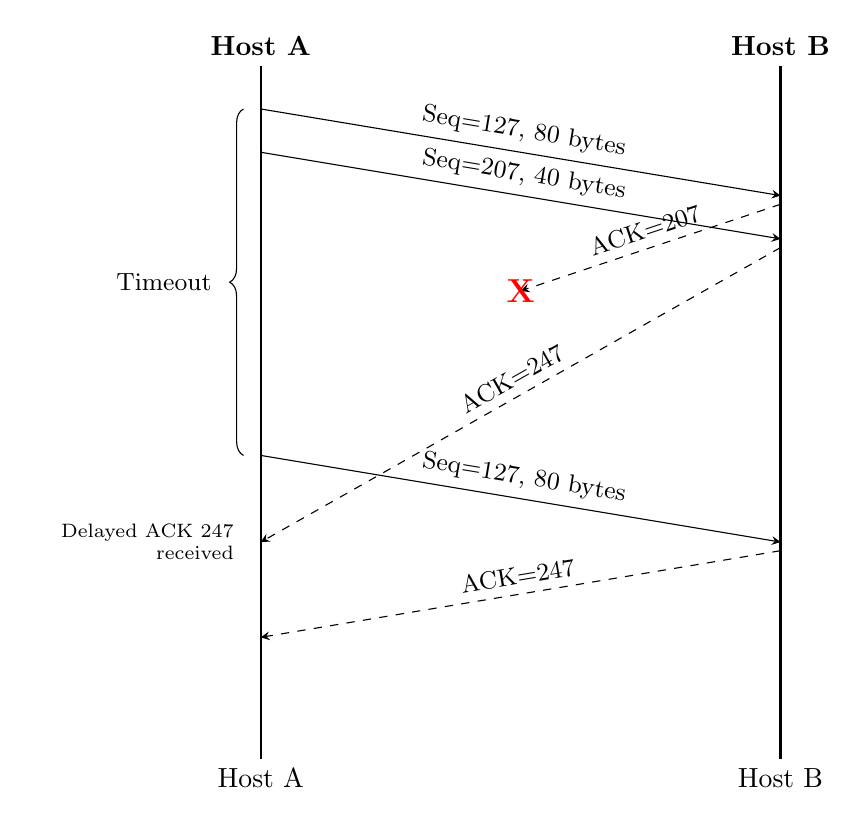
\begin{tikzpicture}[>=stealth, scale=1.1]
		% Draw Host vertical lines
		\draw[thick] (0,0) -- (0,-8) node[below] {Host A};
		\draw[thick] (6,0) -- (6,-8) node[below] {Host B};
		\node[above, font=\bfseries] at (0,0) {Host A};
		\node[above, font=\bfseries] at (6,0) {Host B};

		% Segment 1
		\draw[->] (0,-0.5) -- (6,-1.5) node[midway, above, sloped, font=\small] {Seq=127, 80 bytes};
		% Segment 2
		\draw[->] (0,-1) -- (6,-2) node[midway, above, sloped, font=\small] {Seq=207, 40 bytes};

		% ACK 207 (Lost)
		\draw[->, dashed] (6,-1.6) -- (3,-2.6) node[midway, above, sloped, font=\small] {ACK=207};
		\node[font=\large, text=red] at (3,-2.6) {\textbf{X}}; % Loss indicator

		% ACK 247 (Delayed - arrives after timeout)
		\draw[->, dashed] (6,-2.1) -- (0,-5.5) node[midway, above, sloped, font=\small] {ACK=247};

		% Timeout Brace
		\draw[decorate,decoration={brace,amplitude=5pt,mirror}] (-0.2,-0.5) -- (-0.2,-4.5) node[midway, left=8pt, font=\small] {Timeout};

		% Retransmission Seg 1
		\draw[->] (0,-4.5) -- (6,-5.5) node[midway, above, sloped, font=\small] {Seq=127, 80 bytes};

		% Late ACK 247 arrives right around here
		\node[left, font=\scriptsize, text width=2.5cm, align=right] at (-0.2,-5.5) {Delayed ACK 247\\received};

		% ACK 247 for retransmission
		\draw[->, dashed] (6,-5.6) -- (0,-6.6) node[midway, above, sloped, font=\small] {ACK=247};

	\end{tikzpicture}
\end{center}

\pagebreak
\problem{2}
\question{Consider the TCP procedure for estimating RTT. Suppose that $\alpha=0.1$. Let SampleRTT1 be the most recent sample RTT, let SampleRTT2 be the next most recent sample RTT, and so on.  (a) Express EstimatedRTT in terms of the four sample RTTs.  (b) Generalize your formula for n sample RTTs. (c) For the formula in part (b) let n approach infinity. Comment on why this averaging procedure is called an exponential moving average. }

\answer{
	\textbf{a.} Using the formula $E_{new} = (1-\alpha)E_{old} + \alpha S_{new}$, and assuming we start updating from the oldest sample ($SampleRTT_4$) to the newest ($SampleRTT_1$):
	\begin{align*}
		E_4 & = S_4                                                                           \\
		E_3 & = (1-\alpha)S_4 + \alpha S_3                                                    \\
		E_2 & = (1-\alpha)^2 S_4 + \alpha(1-\alpha) S_3 + \alpha S_2                          \\
		E_1 & = (1-\alpha)^3 S_4 + \alpha(1-\alpha)^2 S_3 + \alpha(1-\alpha) S_2 + \alpha S_1
	\end{align*}
	Substituting $\alpha = 0.1$:
	$EstimatedRTT = 0.9^3 \cdot S_4 + 0.1(0.9^2) \cdot S_3 + 0.1(0.9) \cdot S_2 + 0.1 \cdot S_1$

	\textbf{b.} Generalizing for $n$ sample RTTs (where $S_n$ is the oldest and $S_1$ is the newest):
	$EstimatedRTT = \sum_{j=1}^{n-1} \alpha (1-\alpha)^{j-1} \cdot S_j$

	\textbf{c.} As $n \to \infty$, the weight given to the oldest sample, $(1-\alpha)^{n-1}$, approaches $0$. This procedure is called an exponential moving average (EMA) because the weight given to past samples decays exponentially as they get older (dictated by the $(1-\alpha)^{j-1}$ multiplier). This ensures the formula adapts quickly to recent network conditions while smoothly forgetting very old samples.
}


\pagebreak
\problem{3}
\question{Consider a modification to TCP’s congestion control algorithm. Instead of additive increase, we can use multiplicative increase. A TCP sender increases its window size by a small positive constant a (0 < a < 1) whenever it receives a valid ACK.  Find the functional relationship between loss rate L and maximum congestion window W. Argue that for this modified TCP, regardless of TCP’s average throughput, a TCP connection always spends the same amount of time to increase its congestion window size from W/2 to W.}

\answer{
	In this modification, the window size increases by $a$ for each ACK received. During one Round Trip Time (RTT), approximately $W$ ACKs are received, meaning the window size increases by $aW$. Therefore, after one RTT, the new window size is $W + aW = (1+a)W$. This defines a multiplicative increase per RTT.

	To find the time (in number of RTTs, let's call it $k$) required to increase from $W/2$ to $W$:
	$$ \frac{W}{2} (1+a)^k = W \implies (1+a)^k = 2 \implies k = \frac{\ln(2)}{\ln(1+a)} $$
	Because $k$ depends strictly on the constant $a$ and not on $W$, a TCP connection always spends the exact same number of RTTs (time) to increase its congestion window from $W/2$ to $W$, regardless of its throughput.

	\textbf{Functional relationship between L and W:} The total number of packets sent ($P$) in one cycle (growing from $W/2$ to $W$) is the sum of a geometric series:
	$$ P = \sum_{i=0}^{k} \frac{W}{2}(1+a)^i = \frac{W}{2} \frac{(1+a)^{k+1}-1}{(1+a)-1} $$
	Since $(1+a)^k = 2$, we can substitute this to simplify:
	$$ P = \frac{W}{2} \frac{2(1+a)-1}{a} = \frac{W(2a+1)}{2a} $$
	Assuming $a$ is small, $2a+1 \approx 1$, so $P \approx \frac{W}{2a}$. Because the loss rate $L$ is the inverse of the number of packets sent between losses ($L = 1/P$), we get:
	$$ L = \frac{2a}{W} \implies W = \frac{2a}{L} $$
	Thus, $W$ is inversely proportional to $L$.
}

\pagebreak
\problem{4}
\question{Suppose that the UDP receiver computes the Internet checksum for the received UDP segment and finds that it matches the value carried in the checksum field. Can the receiver be absolutely certain that no bit errors have occurred? Explain. }

\answer{
	No, the receiver cannot be absolutely certain that no bit errors have occurred. The Internet checksum uses 1s complement arithmetic. If there are multiple bit errors that cancel each other out, the checksum will fail to detect them. For example, if a `0` becomes a `1` in one column of a 16-bit word, and a `1` becomes a `0` in that exact same column of another 16-bit word within the segment, the arithmetic sum remains exactly the same, and the checksum will falsely validate the corrupted packet.
}


\problem{5}
\question{Draw the FSM for the receiver side of protocol rdt3.0}

\answer{
	Below is the formal textual representation of the receiver side FSM for the rdt 3.0 (alternating-bit) protocol:

	\textbf{State 1: Wait for 0 from below}
	\begin{itemize}
		\item \textbf{Event:} \texttt{rdt\_rcv(rcvpkt) \&\& notcorrupt(rcvpkt) \&\& has\_seq0(rcvpkt)}
		\item \textbf{Action:} \texttt{extract(rcvpkt, data); deliver\_data(data); make\_pkt(sndpkt, ACK, 0); udt\_send(sndpkt)}
		\item \textbf{Transition:} Move to State 2.
		\item \textbf{Event:} \texttt{rdt\_rcv(rcvpkt) \&\& (corrupt(rcvpkt) || has\_seq1(rcvpkt))}
		\item \textbf{Action:} \texttt{make\_pkt(sndpkt, ACK, 1); udt\_send(sndpkt)}
		\item \textbf{Transition:} Remain in State 1.
	\end{itemize}

	\textbf{State 2: Wait for 1 from below}
	\begin{itemize}
		\item \textbf{Event:} \texttt{rdt\_rcv(rcvpkt) \&\& notcorrupt(rcvpkt) \&\& has\_seq1(rcvpkt)}
		\item \textbf{Action:} \texttt{extract(rcvpkt, data); deliver\_data(data); make\_pkt(sndpkt, ACK, 1); udt\_send(sndpkt)}
		\item \textbf{Transition:} Move to State 1.
		\item \textbf{Event:} \texttt{rdt\_rcv(rcvpkt) \&\& (corrupt(rcvpkt) || has\_seq0(rcvpkt))}
		\item \textbf{Action:} \texttt{make\_pkt(sndpkt, ACK, 0); udt\_send(sndpkt)}
		\item \textbf{Transition:} Remain in State 2.
	\end{itemize}
}

\begin{center}
	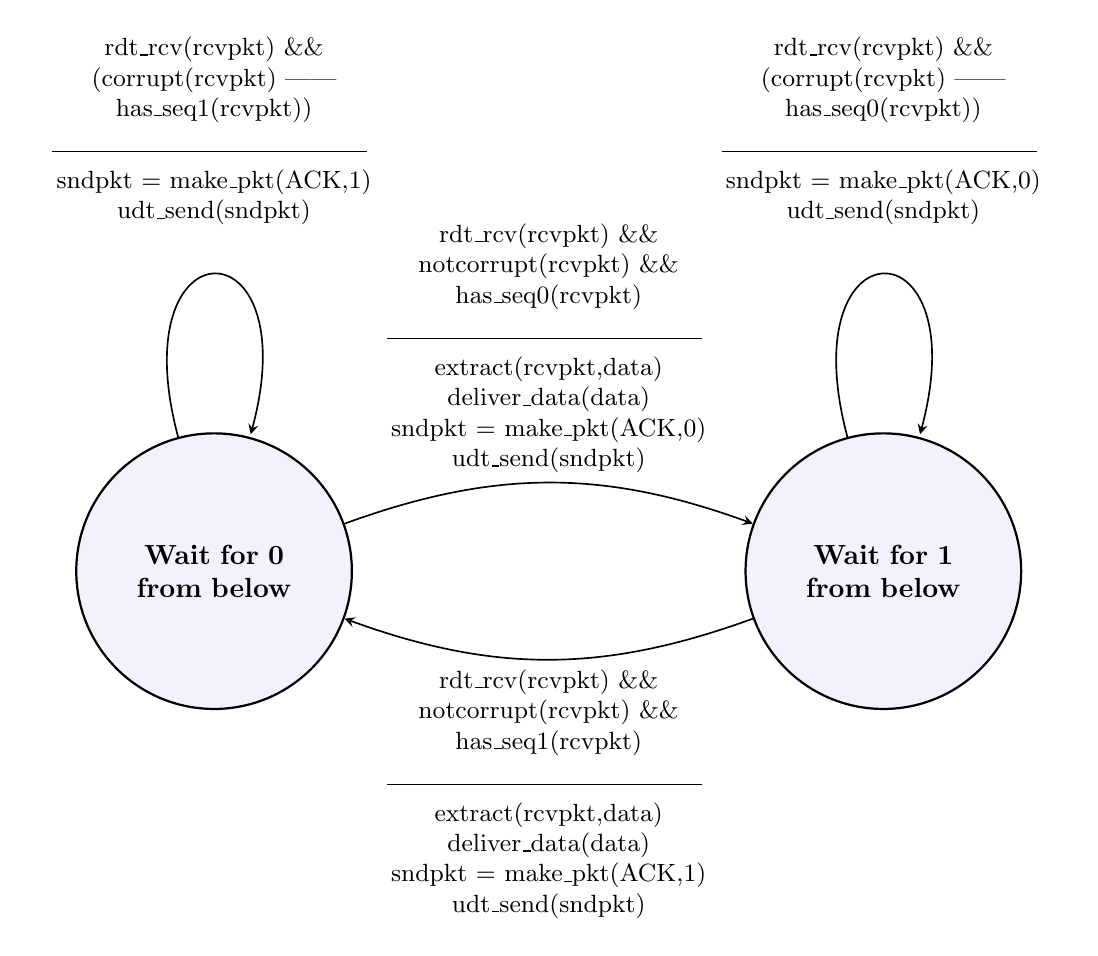
\begin{tikzpicture}[->, >=stealth, auto, node distance=8.5cm, semithick]
		\tikzstyle{state}=[circle, draw, thick, minimum size=3.5cm, text centered, text width=2.5cm, fill=blue!5]

		\node[state] (S0) {\textbf{Wait for 0 from below}};
		\node[state] (S1) [right of=S0] {\textbf{Wait for 1 from below}};

		\path
		(S0) edge [bend left=20] node[above, text width=5cm, align=center, font=\small] {
				rdt\_rcv(rcvpkt) \&\&\\ notcorrupt(rcvpkt) \&\&\\ has\_seq0(rcvpkt) \\
				\vspace{2pt} \rule{4cm}{0.4pt} \vspace{2pt} \\
				extract(rcvpkt,data) \\ deliver\_data(data) \\ sndpkt = make\_pkt(ACK,0) \\ udt\_send(sndpkt)
			} (S1)

		(S0) edge [loop above] node[text width=4.5cm, align=center, font=\small, yshift=0.5cm] {
				rdt\_rcv(rcvpkt) \&\&\\ (corrupt(rcvpkt) ||\\ has\_seq1(rcvpkt)) \\
				\vspace{2pt} \rule{4cm}{0.4pt} \vspace{2pt} \\
				sndpkt = make\_pkt(ACK,1) \\ udt\_send(sndpkt)
			} (S0)

		(S1) edge [bend left=20] node[below, text width=5cm, align=center, font=\small] {
				rdt\_rcv(rcvpkt) \&\&\\ notcorrupt(rcvpkt) \&\&\\ has\_seq1(rcvpkt) \\
				\vspace{2pt} \rule{4cm}{0.4pt} \vspace{2pt} \\
				extract(rcvpkt,data) \\ deliver\_data(data) \\ sndpkt = make\_pkt(ACK,1) \\ udt\_send(sndpkt)
			} (S0)

		(S1) edge [loop above] node[text width=4.5cm, align=center, font=\small, yshift=0.5cm] {
				rdt\_rcv(rcvpkt) \&\&\\ (corrupt(rcvpkt) ||\\ has\_seq0(rcvpkt)) \\
				\vspace{2pt} \rule{4cm}{0.4pt} \vspace{2pt} \\
				sndpkt = make\_pkt(ACK,0) \\ udt\_send(sndpkt)
			} (S1);
	\end{tikzpicture}
\end{center}

\pagebreak
\problem{6}
\question{Answer true or false to the following questions and briefly justify your answer: (a) With the SR protocol, it is possible for the sender to receive an ACK for a packet that falls outside of its current window. (b) With GBN, it is possible for the sender to receive an ACK for a packet that falls outside of its current window. (c) The alternating-bit protocol is the same as the SR protocol with a sender and receiver window size of 1. (d) The alternating-bit protocol is the same as the GBN protocol with a sender and receiver window size of 1.}

\answer{
	\textbf{a. True.} If an ACK is heavily delayed in the network, the sender may have already advanced its window (e.g., due to a timeout causing a retransmission, or other packets being acknowledged). When the heavily delayed ACK finally arrives, its sequence number will fall outside of the sender's newly updated window.

	\textbf{b. True.} Similar to SR, if an ACK in Go-Back-N (GBN) is heavily delayed and the sender's window has already slid forward (e.g., after a timeout and subsequent fresh ACKs), the old, delayed ACK will fall outside the sender's current window boundaries.

	\textbf{c. True.} The Selective Repeat (SR) protocol uses a window size to allow multiple unacknowledged packets. If the window size is restricted to exactly $1$ for both sender and receiver, the sender can only send a single packet and must wait for that specific ACK before advancing the window, which is the exact behavior of the alternating-bit (stop-and-wait) protocol.

	\textbf{d. True.} Go-Back-N (GBN) with a sender window size of $1$ and a receiver window size of $1$ also strictly limits the sender to one unacknowledged packet at a time. This effectively strips away the "Go-Back-N" pipeline and reduces it to a stop-and-wait protocol, identical to the alternating-bit protocol.
}

\end{document}
